\documentclass[a4paper,12pt]{article}

\usepackage{graphicx} % Required for inserting images
\usepackage{amsmath,amssymb,amsfonts}
\usepackage{subcaption}
% -----------------------
% Package Imports
% -----------------------

% Set page margins
\usepackage[a4paper, top=1in, bottom=0.8in, left=1.1in, right=0.8in]{geometry}

% Use Times New Roman font
\usepackage{times}





% Set page margins
\usepackage[a4paper, top=1in, bottom=0.8in, left=1.1in, right=0.8in]{geometry}


% Add page numbering
\pagestyle{plain}

% Enable graphics inclusion
\usepackage{graphicx}
\usepackage{float}
% Enable code listings
\usepackage{listings}
\usepackage{xcolor} % For customizing code colors
\setlength{\parindent}{0pt}
\usepackage{multirow}

\setlength{\parindent}{0pt}
\usepackage{titlesec} % To customize section font size
\titleformat{\section}
{\normalfont\fontsize{14}{16}\bfseries}{\thesection}{1em}{}

\titleformat{\subsection}
{\normalfont\fontsize{14}{16}\bfseries}{\thesubsection}{1em}{}

\begin{document}
	\section{Experiment No. 7}
	
	\section{Experiment Title }
	Observation of Load Characteristics of three phase Synchronous motor.
	
	\section{Objective}
	
	The objectives of this lab are as follows:
	\begin{itemize}
		\item 	To observe the variation of armature current with mechanical load.
		\item 	To analyze the effect of excitation on motor performance under varying loads
		
		
		
	\end{itemize}
	
	\section{Theory}
	
	
A synchronous motor is a type of AC motor in which the rotor rotates at exactly the same speed as the stator's rotating magnetic field. This constant speed is called the \textbf{synchronous speed} and is given by:

\begin{equation}
	N_s = \frac{120f}{P}
\end{equation}

where,  
$N_s$ = synchronous speed in rpm,  
$f$ = supply frequency in Hz,  
$P$ = number of poles of the motor.

Unlike induction motors, the synchronous motor does not experience slip under steady-state conditions and maintains constant speed regardless of load variations, as long as it remains in synchronism.

\subsection*{Starting Mechanism}

When a three-phase AC supply is applied to the stator, it produces a rotating magnetic field. However, the rotor initially cannot lock into this field directly. Therefore, auxiliary starting mechanisms, such as damper windings (similar to squirrel cage rotors) or external prime movers, are used to bring the rotor speed close to synchronous speed. Once this condition is achieved, the rotor's magnetic field locks with the stator's rotating field, allowing synchronous operation.

\subsection*{Voltage Equation}

The per-phase voltage equation of a synchronous motor is:

\begin{equation}
	V_\phi = E_A + I_A R_A + jI_A X_s
\end{equation}

where,  
$V_\phi$ = stator terminal voltage per phase,  
$E_A$ = internal generated EMF per phase,  
$I_A$ = armature current per phase,  
$R_A$ = armature resistance,  
$X_s$ = synchronous reactance.

If the armature resistance $R_A$ is neglected, the equation simplifies to:

\begin{equation}
	V_\phi = E_A + jI_A X_s
\end{equation}

\subsection*{Load Characteristics}

As the mechanical load on the motor shaft changes, the synchronous motor exhibits specific load-dependent behaviors:

\begin{enumerate}
	\item \textbf{Constant Speed:} The rotor speed remains constant and equal to synchronous speed regardless of load changes. This is a defining characteristic of synchronous motors.
	
	\item \textbf{Torque Angle ($\delta$):} The torque angle $\delta$ is the angle between the stator magnetic field and the rotor magnetic field. As the load increases, the motor increases torque by increasing $\delta$. If $\delta$ exceeds a critical value (associated with pull-out torque), the motor loses synchronism.
	
	\item \textbf{Armature Current ($I_A$):} With increasing mechanical load, the armature current increases to meet the required torque. This current increase is not due to a change in speed but is driven by torque demand.
	
	\item \textbf{Power Factor Variation:} The power factor of a synchronous motor is dependent on the level of field excitation:
	\begin{itemize}
		\item Under-excited ($E_A < V_\phi$): Lagging power factor.
		\item Normal excitation ($E_A = V_\phi$): Unity power factor.
		\item Over-excited ($E_A > V_\phi$): Leading power factor.
	\end{itemize}
	As load increases, the power factor shifts further in the lagging direction for under-excited machines and less leading for over-excited ones.
\end{enumerate}

\subsection*{Power and Torque Expression}

The electromagnetic torque developed by a synchronous motor is given by:

\begin{equation}
	T = \frac{3EV}{\omega_s X_s} \sin\delta
\end{equation}

where,  
$E$ = internal EMF,  
$V$ = terminal voltage,  
$\omega_s$ = synchronous angular speed,  
$X_s$ = synchronous reactance,  
$\delta$ = torque angle.
\begin{figure}[H]
	\centering
	\includegraphics[width=0.7\linewidth]{"C:/Users/win-11/Pictures/Screenshots/Screenshot 2025-06-17 105308"}
	\caption{The phasor diagram of increase load on the operation of a synchronous motor}
	\label{fig:screenshot-2025-06-17-105308}
\end{figure}

\subsection{Effect of Load on Phasor Diagram}

As the load increases:
\begin{itemize}
	\item The torque angle $\delta$ increases.
	\item The vector $jX_s I_A$ becomes longer to maintain the voltage relation between $E_A$ and $V_\phi$.
	\item The armature current $I_A$ increases in magnitude.
	\item The power factor angle $\theta$ changes accordingly—becoming less leading or more lagging.
\end{itemize}

Since the field current ($I_F$) and supply frequency remain constant, the magnitude of $E_A = K\phi\omega$ remains unchanged. However, as $\delta$ increases, $E_A$ swings further below the horizontal axis in the phasor diagram. The tip of $jX_s I_A$ must reach from the tip of $E_A$ to $V_\phi$, leading to an increase in $I_A$ and a change in the power factor.

\section{Circuit Diagram}
\begin{figure}[H]
	\centering
	\	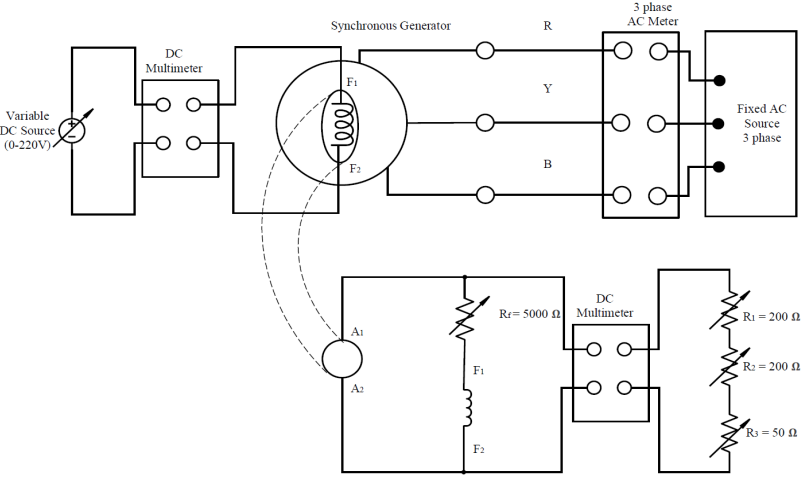
\includegraphics[width=1\textwidth]{Images/1}
	\caption{Experimental Setup of Synchronous Motor under load variations}
	
\end{figure}



	\newpage
	\section{Required Apparatus}
	
	
	\begin{enumerate}
		\item \textbf{DC Motor}
		\begin{enumerate}
			\item Power: 300W , Speed: 3000 rpm
			\item Voltage: 220V
			\item \textbf{Excitation (Series)}: D1-D2, Current: 1.9A, \textbf{Excitation (Separate)}: F1-F2, Current: 1.8A, Excitation Voltage: 220V, Excitation Current: 0.1A
			
		\end{enumerate}
		
		\item \textbf{Synchronous Motor}
		\begin{enumerate}
			\item Power: 350W ,Power Factor: $\cos\phi = 1$ ,Speed: 3000 rpm
			
			\item Voltage: 400V (star) / 230V (delta) ,Current: 0.7A (star) / 1.2A (delta) 
			\item Excitation Voltage: 220V ,Excitation Current: 0.45A
			
		\end{enumerate}
		
		\item \textbf{Resistors}
		\begin{enumerate}
			\item 50$\Omega$: Power = 500W, Current = 3.16A
			\item 200$\Omega$: Power = 500W, Current = 1.58A
			\item 5000$\Omega$: Power = 500W, Current = 0.31A
		\end{enumerate}
		
		\item \textbf{Tachometer}
		\begin{enumerate}
			\item For 0.6V/rev: 300V at 5000 RPM , For 2mV/rev: 10V at 5000 RPM
			\item Maximum Current: 0.07A
			\item Maximum Speed: 5000 RPM
		\end{enumerate}
		
		\item \textbf{AC Multimeter}
		\begin{enumerate}
			\item 500V AC RMS
			\item 5A
		\end{enumerate}
	\end{enumerate}
	\newpage
	\section{Data Table}
	\begin{table}[H]
		\centering
		\caption{Experimental Data of Synchronous Motor under load variations }
		\begin{tabular}{|c|c|c|c|c|}
			\hline
			\textbf{\begin{tabular}[c]{@{}c@{}}SL   \\ No.\end{tabular}} & \textbf{\begin{tabular}[c]{@{}c@{}}Load Current, \\ I\_A (A)\end{tabular}} & \textbf{\begin{tabular}[c]{@{}c@{}}Active   Power, \\ P (W)\end{tabular}} & \textbf{\begin{tabular}[c]{@{}c@{}}Reactive   Power,\\     Q (VAR)\end{tabular}} & \textbf{\begin{tabular}[c]{@{}c@{}}Motor   Current, \\    I\_M (A)\end{tabular}} \\ \hline
			01.                                                          & 0.197                                                                      & 28.0                                                                      & 71.4                                                                             & 0.304                                                                            \\ \hline
			02.                                                          & 0.206                                                                      & 30.5                                                                      & 71.2                                                                             & 0.343                                                                            \\ \hline
			03.                                                          & 0.205                                                                      & 30.6                                                                      & 72.2                                                                             & 0.338                                                                            \\ \hline
			04.                                                          & 0.211                                                                      & 30.4                                                                      & 71.5                                                                             & 0.334                                                                            \\ \hline
			05.                                                          & 0.212                                                                      & 29.7                                                                      & 71.6                                                                             & 0.339                                                                            \\ \hline
			06.                                                          & 0.210                                                                      & 28.3                                                                      & 72.3                                                                             & 0.338                                                                            \\ \hline
			07.                                                          & 0.205                                                                      & 28.6                                                                      & 71.9                                                                             & 0.336                                                                            \\ \hline
			08.                                                          & 0.202                                                                      & 29.1                                                                      & 70.9                                                                             & 0.335                                                                            \\ \hline
			09.                                                          & 0.195                                                                      & 28.9                                                                      & 71.5                                                                             & 0.332                                                                            \\ \hline
			10.                                                          & 0.104                                                                      & 28.9                                                                      & 71.1                                                                             & 0.333                                                                            \\ \hline
			11.                                                          & 0.203                                                                      & 28.4                                                                      & 70.2                                                                             & 0.331                                                                            \\ \hline
			12.                                                          & 0.208                                                                      & 28.1                                                                      & 70.7                                                                             & 0.329                                                                            \\ \hline
			13.                                                          & 0.215                                                                      & 28.6                                                                      & 70.6                                                                             & 0.331                                                                            \\ \hline
			14.                                                          & 0.218                                                                      & 28.6                                                                      & 70.2                                                                             & 0.334                                                                            \\ \hline
		\end{tabular}
	\end{table}
	
	\section{Discussion}

In this experiment, the load characteristics of a synchronous motor were tested under a fixed supply voltage. The motor was operated at a constant synchronous speed throughout the test, indicating that proper synchronization had been achieved.

As mechanical load was gradually increased, corresponding load and motor currents were recorded. It was observed that the motor current varied slightly with load, implying that the increments in mechanical load were relatively small and that the field excitation had likely been maintained at a constant level. Active and reactive power values remained nearly unchanged, which suggested minimal fluctuation in the power factor.

No instance of loss of synchronism was encountered during the experiment. This indicated that the motor had been operated within its stability limit and that the pull-out torque had not been exceeded. 

Overall, the synchronous motor’s behavior under varying load conditions exhibited stable electrical performance and confirmed the theoretical expectation of constant-speed operation, regardless of changes in load.

	
	
\end{document}
